\documentclass[../main.tex]{subfiles}

\begin{document}

\section{Results}

\subsection{Fashion-MNIST}
\subsubsection{CNN}
The training session for the CNN on the Fashion-MNIST dataset initially developed promisingly. However, the loss shown in the validation set quickly increased in the last epochs, as shown in figure \ref{fig:fashion_mnist_cnn_history}

\begin{figure}[H]
    \begin{subfigure}{.5\textwidth}
        \centering
        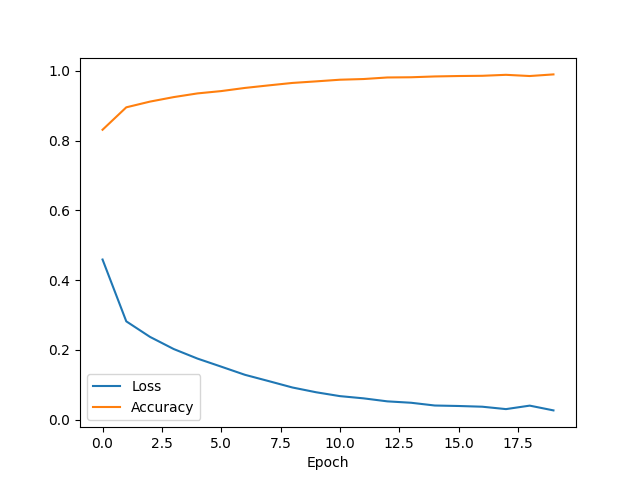
\includegraphics[width=1.1\linewidth]{doc/assets/fashion_mnist_train_history.png}
    \end{subfigure}
    \begin{subfigure}{.5\textwidth}
        \centering
        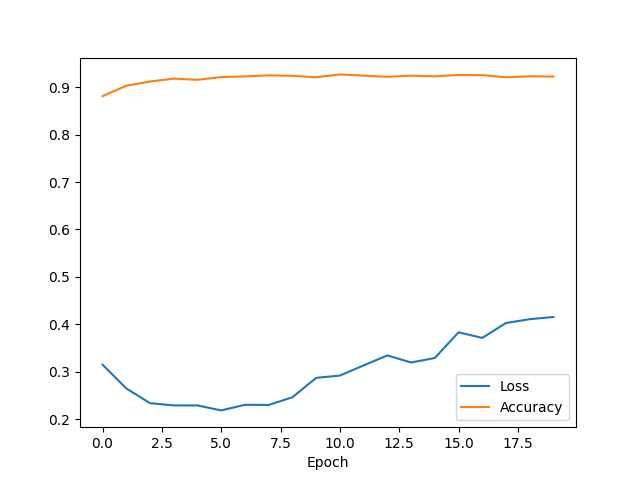
\includegraphics[width=1.1\linewidth]{doc/assets/fashion_mnist_val_history.png}
    \end{subfigure}
    \caption{History of loss and accuracy of the training and validation set as they develop through the epochs.}
    \label{fig:fashion_mnist_cnn_history}
\end{figure}


\subsubsection{Logistic regression}
The logistic regression model was applied on the mnist fashion dataset. The logistic regression resulted in an accuracy of 84\% when applied to the test set. The accuracy from the train set was 88\%. The confusion matrix which shows the accuracy of each article can be seen in figure \ref{fig:logreg_mnist_cm}.
\begin{figure}[H]
    \centering
    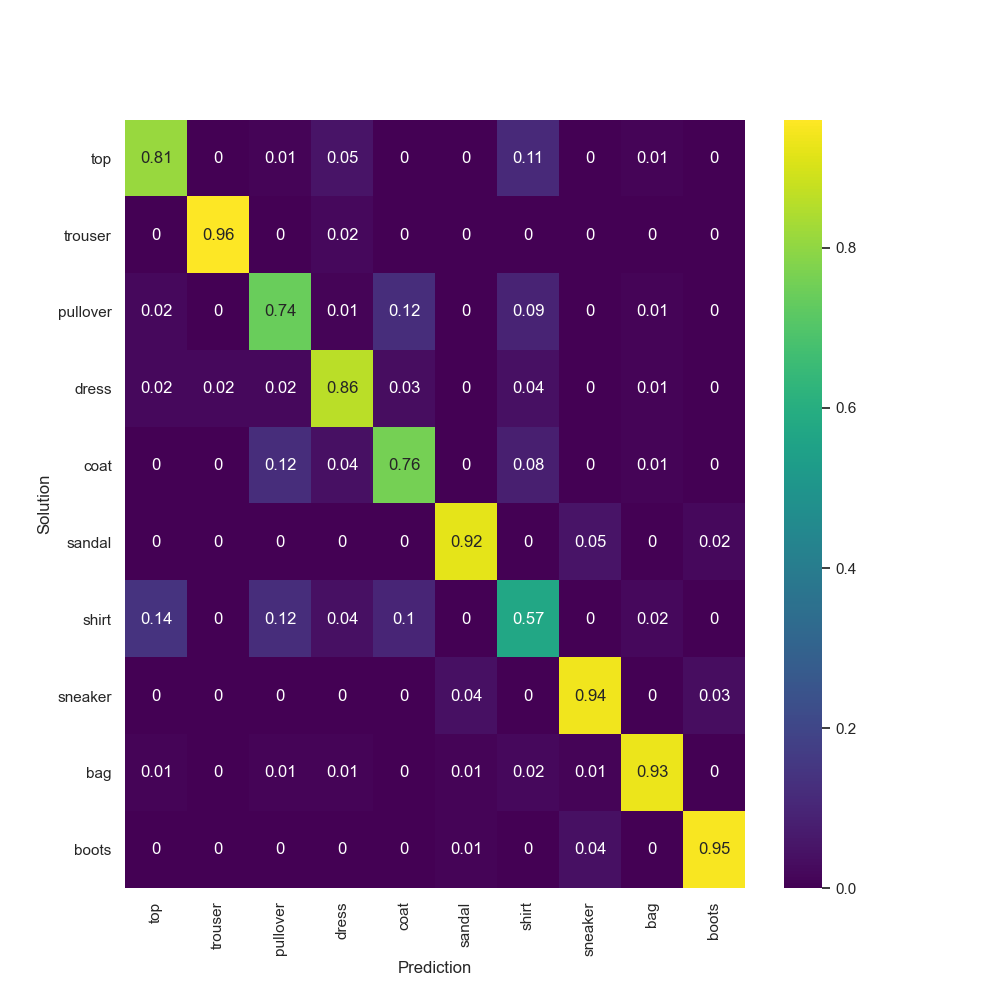
\includegraphics[width=0.8\textwidth]{doc/assets/logreg_fashion_heatmap_accuracy84.png}
    \caption{The confusion matrix after using logistic regression to classify the fashion mnist. The matrix shows the accuracy of the model within each predicted class}
    \label{fig:logreg_mnist_cm}
\end{figure}

Some of the missclassified pictures from using logistic regression on the fashion mnist dataset can be seen in figure \ref{fig:missclassified_logreg_fashion}

\begin{figure}[H]
    \centering
    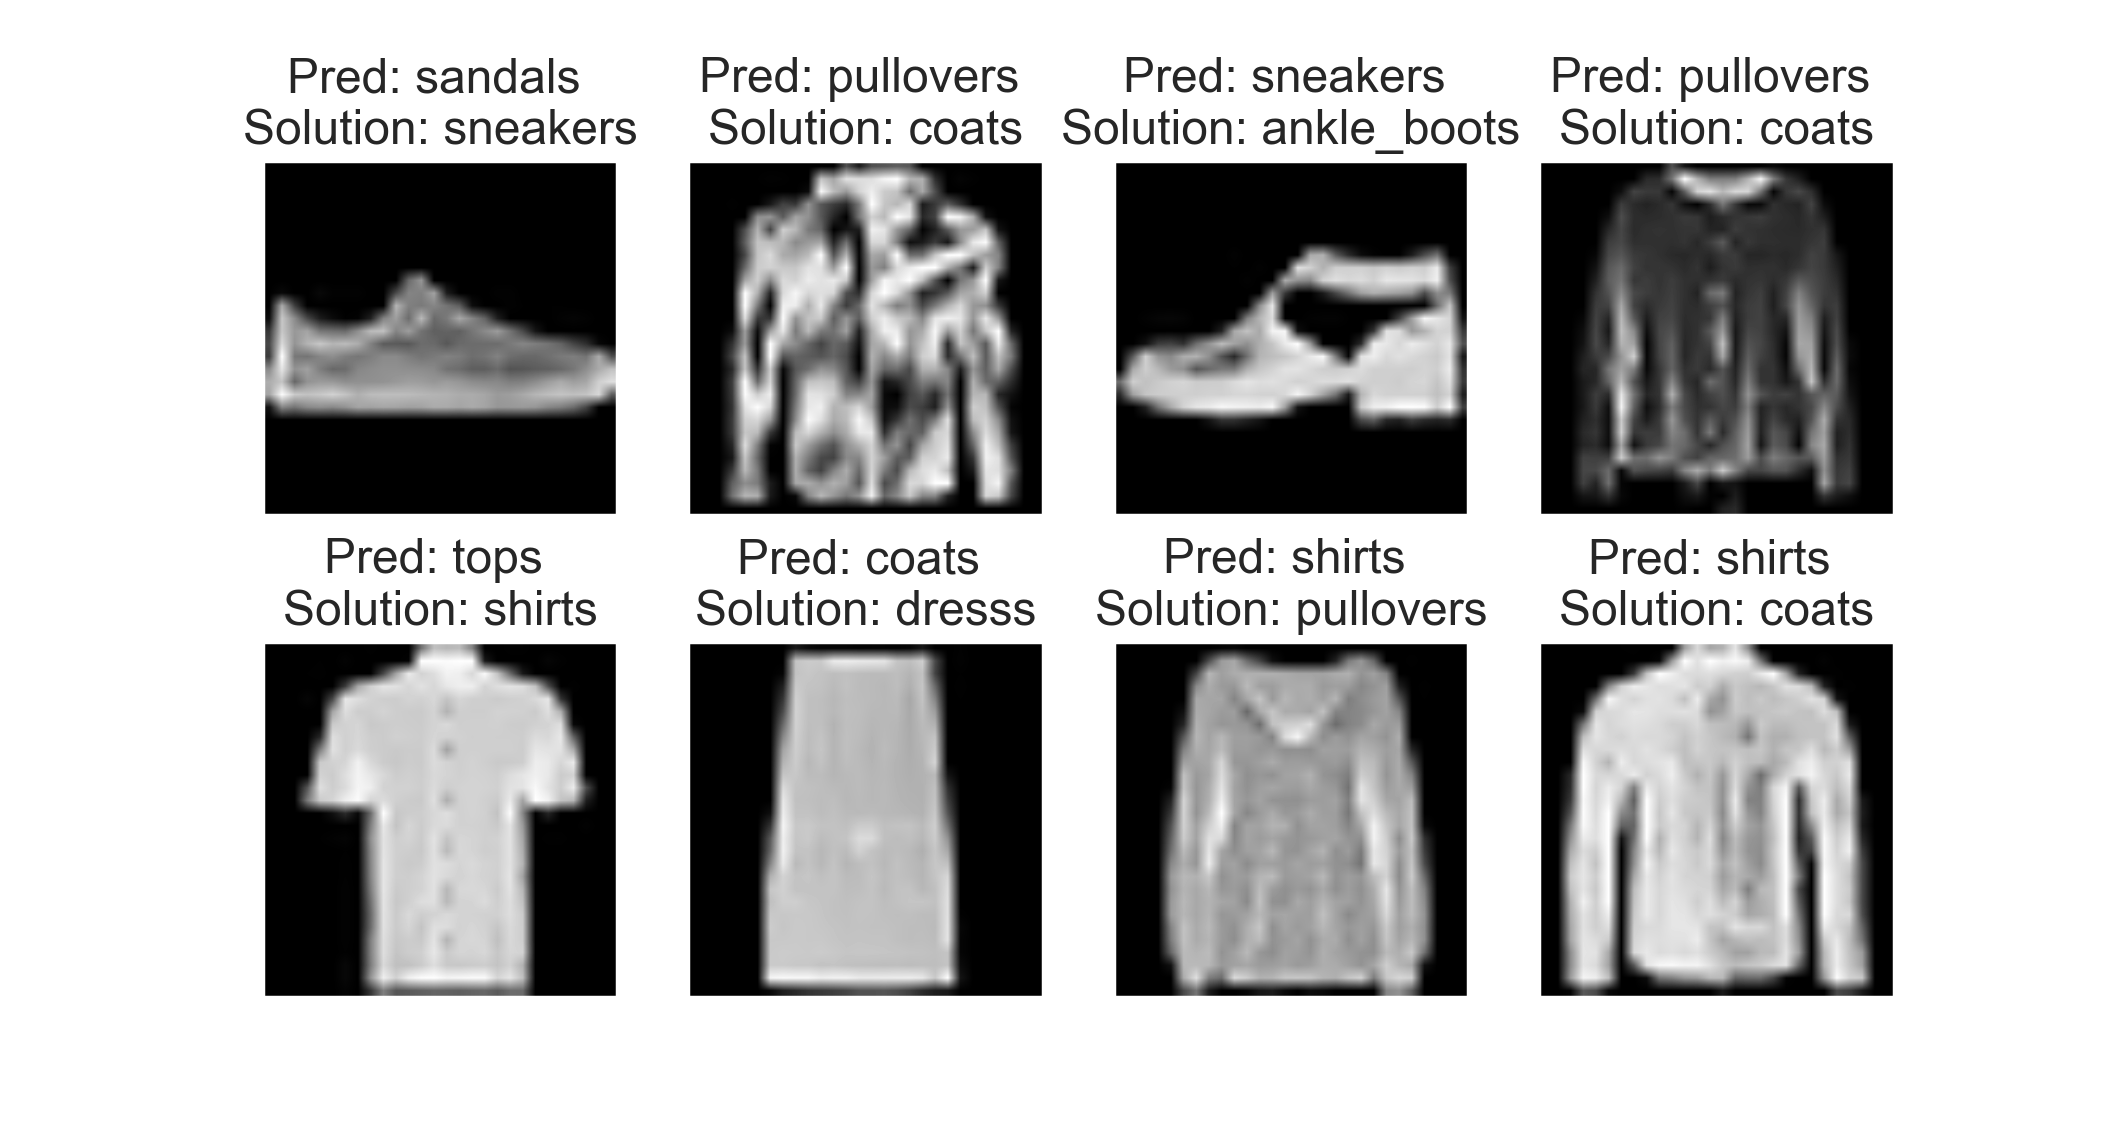
\includegraphics[width=0.8\textwidth]{doc/assets/logreg_missclassified_fasion.png}
    \caption{Some missclassified images from the mnist fashion dataset, predicted by logistic regression}
    \label{fig:missclassified_logreg_fashion}
\end{figure}

\subsection{Face mask detection}
\subsubsection{CNN}
% Some text about training history. The validation history is utter bullshit, but that is hopefully fixed soon.

\begin{figure}[H]
    \begin{subfigure}{.5\textwidth}
        \centering
        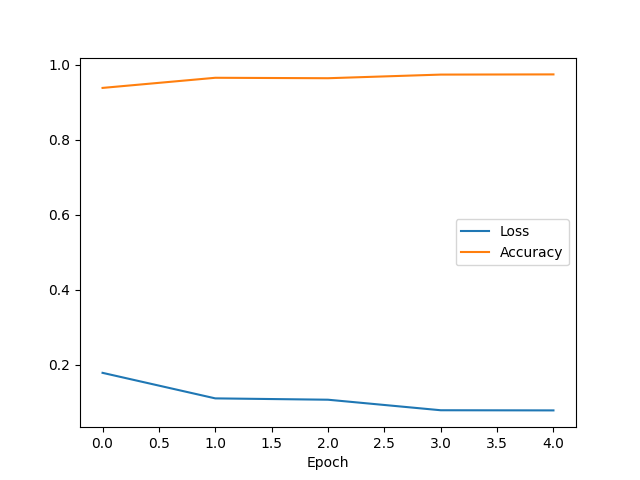
\includegraphics[width=1.1\linewidth]{doc/assets/facemasks_train_history.png}
    \end{subfigure}
    \begin{subfigure}{.5\textwidth}
        \centering
        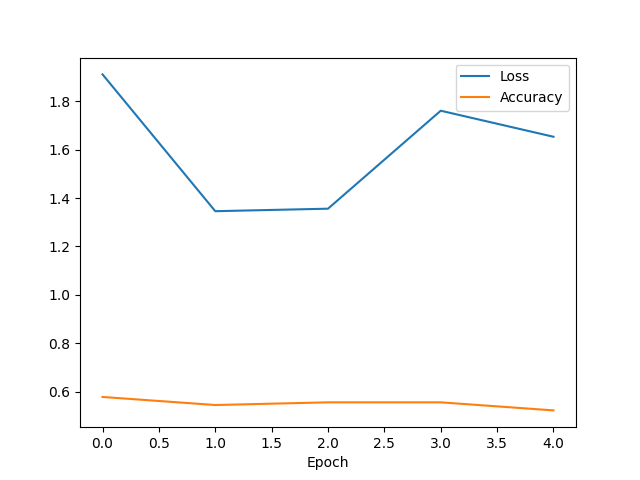
\includegraphics[width=1.1\linewidth]{doc/assets/facemasks_val_history.png}
    \end{subfigure}
    \caption{History of loss and accuracy of the training and validation set as they develop through the epochs.}
    \label{fig:facemasks_cnn_history}
\end{figure}

After training on the dataset, our model classified a collection of real pictures of people with facemasks. 

In addition to using the supplied testing set, we snapped a couple of pictures of ourselves to test the network on. Here are some examples and the results the network provided.


\subsubsection{Logistic regression}
The logistic regression model was applied on the face mask dataset. The logistic regression resulted with an accuracy score of 48\% when applied to the test set. The confusion matrix which shows the accuracy of the predicted classifications can be seen in figure \ref{fig:logreg_facemask_cm}. Some of the miss classified images can be seen in figure \ref{fig:missclassified_logreg_facemask}

\begin{figure}[H]
    \centering
    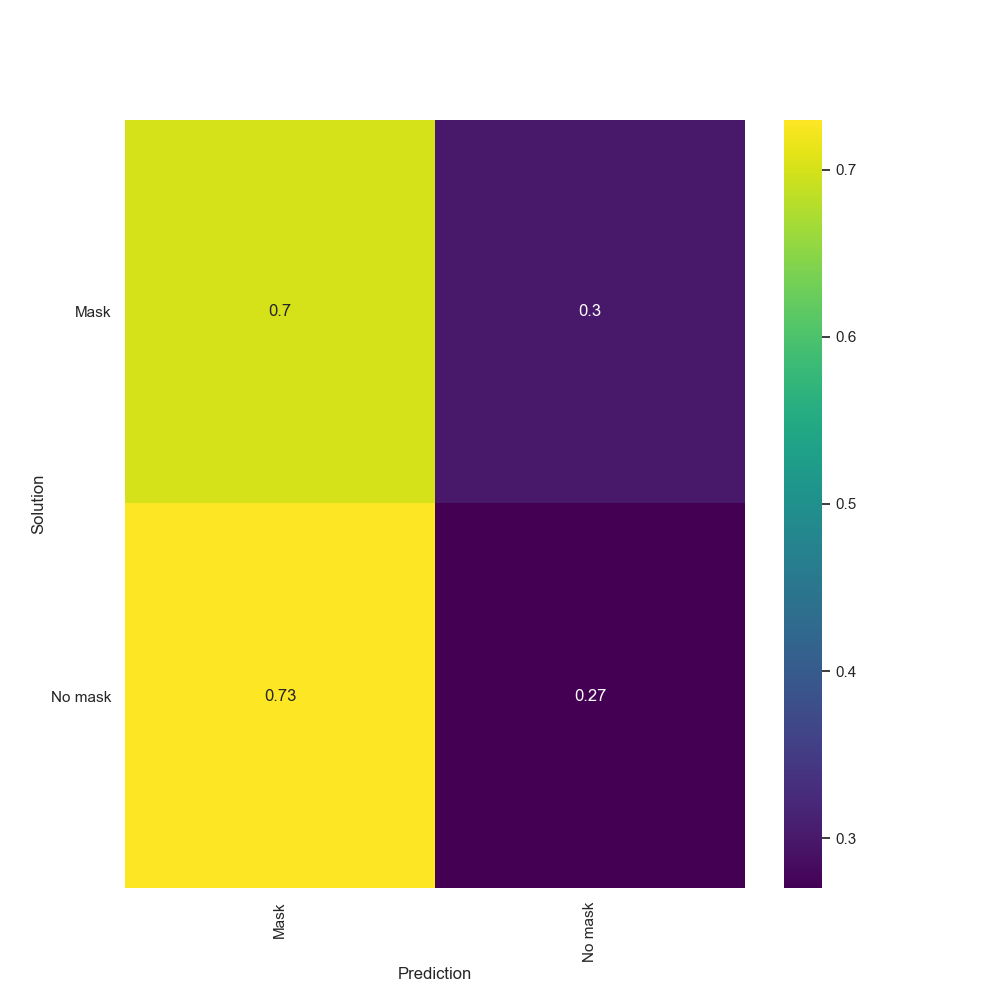
\includegraphics[width=0.8\textwidth]{doc/assets/logreg_mask_heatmap_accuracy48_original_testset.png}
    \caption{The confusion matrix after using logistic regression to classify the face mask detection dataset. The matrix shows the accuracy of the model within each predicted class}
    \label{fig:logreg_facemask_cm}
\end{figure}

\begin{figure}[H]
    \centering
    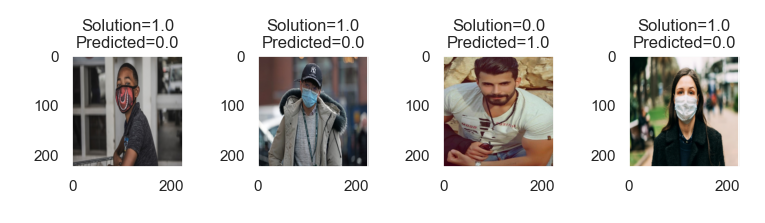
\includegraphics[width=0.8\textwidth]{doc/assets/logreg_missclassified_facemask.png}
    \caption{Some miss classified images from the facemask detection dataset, predicted by logistic regression}
    \label{fig:missclassified_logreg_facemask}
\end{figure}


Since the dataset consisted of images of people with facemasks edited on instead of wearing real physical masks, the model was tested on a few pictures taken by ourself to check how the model performed after training. The results can be seen in figure \ref{fig:logreg_real_pics}

\begin{figure}[H]
    \centering
    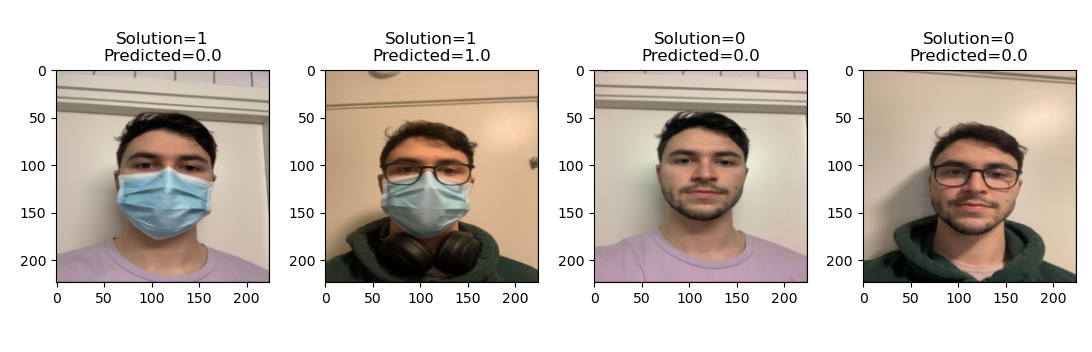
\includegraphics[width=0.8\textwidth]{doc/assets/log_reg_real_pics.png}
    \caption{Pictures taken by ourselves to test the model. The model predicted three out of four pictures correct}
    \label{fig:logreg_real_pics}
\end{figure}


\end{document}